%%%%%%%%%%%%%%%%%%%%%%%%%%%%%%%%%%%%%%%%%%%%%%%%%%%%%%%%%%%%%%%%%%%%%%
% How to use writeLaTeX: 
%
% You edit the source code here on the left, and the preview on the
% right shows you the result within a few seconds.
%
% Bookmark this page and share the URL with your co-authors. They can
% edit at the same time!
%
% You can upload figures, bibliographies, custom classes and
% styles using the files menu.
%
%%%%%%%%%%%%%%%%%%%%%%%%%%%%%%%%%%%%%%%%%%%%%%%%%%%%%%%%%%%%%%%%%%%%%%

\documentclass[12pt]{article}

\usepackage{sbc-template}
\usepackage{booktabs}
\usepackage{url}  % Necessário para exibir URLs corretame
\usepackage{booktabs} % Para melhor formatação da tabela
\usepackage{tabularx} % Para controle de largura da tabela

\usepackage{graphicx,url}

%\usepackage[brazil]{babel}   
\usepackage[utf8]{inputenc}  

     
\sloppy

\title{Algoritmos II - Trabalho Prático 2\\  Soluções para Caixeiro Viajante}

\author{Lucas Rafael Costa Santos\inst{1}, Lucca Alvarenga de Magalhães Pinto\inst{2}}


\address{Departamento de Ciência da Computação -- Universidade Federal de Minas Gerais (UFMG)\\
Belo Horizonte -- MG -- Brazil
}

\begin{document} 

\maketitle

\begin{abstract}
This work presents the implementation of 3 algorithms, an exact solution, based on the Branch-and-Bound algorithm, and two approximate solutions, the Twice-Around-the-Tree algorithm and the Christofides algorithm, for the Traveling Salesman Problem in its Euclidean variation, where the cost function is based on the Euclidean distance in 2D between the points.
\end{abstract}
     
\begin{resumo} 
Esse trabalho apresenta a implementação de 3 algoritmos, uma solução exata, baseada no algoritmo Branch-and-Bound, e duas soluções aproximadas, o algoritmo Twice-Around-the-Tree e o algoritmo de Christofides, para o Problema do Caixeiro Viajante em sua variação euclidiana, onde a função de custo é baseada na distância euclidiana em 2D entre os pontos. 
\end{resumo}

\section{Introdução } \label{sec:firstpage}

O Problema do Caixeiro Viajante (TSP - Traveling Salesman Problem) é um dos problemas mais clássicos e estudados em otimização combinatória e teoria dos grafos. Dado um conjunto de cidades e as distâncias entre cada par de cidades, o objetivo do TSP é encontrar a rota mais curta que visita todas as cidades exatamente uma vez e retornar à cidade de origem. Esse problema é classificado como um problema NP-difícil, o que implica que, não se conhece um algoritmo que resolva todas as instâncias em tempo polinomial em Máquina de Turing Determinística.

Neste trabalho, iremos tratar soluções para uma variante desse problema, o TSP Euclidiano, no qual as cidades são representadas por pontos em um plano cartesiano bidimensional, e as distâncias entre elas são calculadas utilizando a distância euclidiana. Assim, a diferença fundamental entre o TSP geral e o Euclidiano reside na forma como as distâncias entre as cidades são definidas, de forma que, no primeiro as distâncias podem ser arbitrárias, enquanto no segundo as distâncias seguem as regras da geometria euclidiana.

Foram implementados 3 algoritmos para solucionar o problema do caixeiro viajante geométrico: o algoritmo Branch-and-Bound, uma solução exata, e os algoritmos de Christofides e Twice-Around-the-Tree, duas soluções aproximadas ao problema. O objetivo principal deste relatório é analisar essas implementações, detalhando cada uma e justificando as estruturas de dados usadas, e realizando experimentos com base nas instâncias de testes compiladas na biblioteca TSPLIB, fazer uma avaliação de desempenho dos algoritmos, considerando aspectos como tempo de execução, consumo de espaço e qualidade das soluções.


\section{Implementações}

As implementações foram desenvolvidas em Python e utilizam as bibliotecas padrão, além de pacotes como numpy, networkx e pandas. A biblioteca networkx foi escolhida pela eficiência e clareza ao lidar com estruturas de grafos. As subseções a seguir detalham os algoritmos implementados, destacando suas principais características e abordagens.

\subsection{Branch-and-Bound}

O algoritmo Branch-and-Bound foi implementado para encontrar a solução ótima do problema utilizando estratégias de poda. A abordagem organiza os nós em uma árvore de busca, explorando-os de maneira best-first com uma fila de prioridade baseada em heap. A principal ideia é evitar calcular caminhos desnecessários ao determinar limites inferiores (bounds) que ajudam a descartar ramos inviáveis.

\subsubsection{Estrutura e Funcionamento}

Cada nó da árvore armazena informações cruciais para a busca: o custo total até aquele ponto, o nível na árvore (indicando a profundidade da busca), a sequência de vértices já visitados e um limite inferior para o custo total de qualquer solução que possa ser alcançada a partir daquele nó. Esse limite inferior, serve como um guia para a busca, permitindo descartar ramos da árvore que certamente não levarão à solução ótima.

A busca inicia-se a partir do nó raiz, representando o estado inicial e a cada iteração, o algoritmo remove da fila de prioridade o nó com o menor limite inferior e explora seus nós filhos. Ao expandir um nó, são gerados novos nós, cada um correspondendo a uma nova escolha de vértice a ser visitado. Se um nó representar um ciclo completo (isto é, todos os vértices foram visitados), sua solução é comparada com a melhor solução encontrada até então e, se for melhor, passa a ser a nova solução ótima.

\subsubsection{Poda}

A eficiência do algoritmo está diretamente ligada à capacidade de podar ramos da árvore que não conduzem à solução ótima. A poda é realizada ao comparar o limite inferior de um nó com o custo da melhor solução conhecida. Se o limite for maior que o custo da melhor solução, o ramo é descartado, pois qualquer solução completa a partir desse nó terá um custo maior.

\subsubsection{Complexidade}

Embora o Branch-and-Bound garanta encontrar a solução ótima, sua complexidade computacional é exponencial em relação ao número de cidades. Isso significa que o tempo de execução pode crescer rapidamente para instâncias maiores, limitando sua aplicação prática em alguns casos.

Em resumo, o Branch-and-Bound é um algoritmo poderoso para resolver o TSP, mas sua eficiência depende da qualidade da heurística utilizada para calcular os limites inferiores e da capacidade de podar eficientemente a árvore de busca.

\subsection{Twice-Around-The-Tree}

Oe algoritmo Twice-Around-The-Tree aproxima soluções para problema TSP em grafos euclidianos, oferecendo uma solução com custo no máximo duas vezes o custo ótimo. Para isso, ele se baseia na construção de uma Árvore Geradora Mínima (AGM) e em um caminhamento em pré-ordem para formar o ciclo.

\subsubsection{Funcionamento}

Inicialmente, é construída uma Árvore Geradora Mínima (AGM) a partir do grafo completo que representa o problema, utilizando as ferramentas presentes na biblioteca NetworkX. Em seguida, a partir de um vértice raiz arbitrário na AGM, é realizado um caminhamento em pré-ordem, de modo que, essa travessia visite cada vértice da árvore exatamente uma vez, gerando uma sequência de vértices que forma um caminho. Para obter então, um ciclo Hamiltoniano (que passa por todos os vértices exatamente uma vez), o vértice inicial é adicionado ao final do caminho obtido na etapa anterior. Por fim, o custo total da solução é calculado somando os pesos das arestas que compõem o ciclo. 

\subsubsection{Vantagens e Complexidade:}

Uma das principais vantagens do algoritmo Twice-Around-the-Tree é sua baixa complexidade computacional. A etapa que domina o tempo de execução é a construção da AGM, que pode ser realizada em tempo O(n² log n), onde n é o número de vértices. Essa característica o torna aplicável a problemas de grande porte.

Embora não garanta a solução ótima, o algoritmo oferece uma aproximação razoável para o problema do caixeiro viajante, de forma que, a qualidade da solução obtida depende da estrutura do grafo, mas em geral o algoritmo consegue encontrar soluções com um custo próximo ao ótimo.

Portando, é possível notar que o algoritmo Twice-Around-the-Tree é uma ferramenta simples e eficiente para obter soluções aproximadas para o problema do caixeiro viajante, sendo sua baixa complexidade e facilidade de implementação fatores que o tornam uma opção atraente para diversas aplicações práticas.

\subsection{Christofides}

O algoritmo de Christofides representa um avanço significativo na busca por soluções aproximadas para o problema do caixeiro viajante. Ele combina a simplicidade do algoritmo Twice-Around-the-Tree com uma técnica mais sofisticada para obter um fator de aproximação menor, garantindo assim soluções de maior qualidade.

\subsubsection{Funcionamento}
Assim como no algoritmo Twice-Around-the-Tree, inicia-se construindo uma árvore geradora mínima para o grafo completo que representa o problema, a qual conecta todos os vértices com o menor custo total possível. A partir disso então, identificam-se os vértices da AGM que possuem grau ímpar, os quais serão cruciais para a próxima etapa.

Com os vértices de grau ímpar, constrói-se um subgrafo induzido e calcula-se um emparelhamento perfeito (conjunto de arestas que emparelha todos os vértices do subgrafo, sem que nenhuma aresta compartilhe um vértice com outra) de menor peso. Em seguida, as arestas da AGM e as arestas do emparelhamento mínimo são combinadas para formar um multigrafo. Então, utilizando um algoritmo eficiente para encontrar ciclos Eulerianos em multigrafos, obtemos um ciclo que percorre cada aresta do multigrafo exatamente uma vez. O ciclo Euleriano obtido geralmente contém vértices repetidos, dessa forma, para obter um ciclo Hamiltoniano (que passa por cada vértice exatamente uma vez), eliminamos os subcaminhos repetidos e ajustamos o ciclo para incluir apenas os vértices únicos.

\subsubsection{Vantagens e Complexidade:}

Ao adicionar a etapa do emparelhamento mínimo, o algoritmo de Christofides garante um fator de aproximação de 1,5, o que significa que a solução encontrada é no máximo 50\% maior que a solução ótima.

A complexidade do algoritmo é dominada pela construção da AGM e pelo cálculo do emparelhamento mínimo. Embora seja mais complexa que o Twice-Around-the-Tree, ainda é polinomial e eficiente para muitos problemas práticos.

Em resumo, o algoritmo de Christofides oferece um excelente equilíbrio entre a qualidade da solução e a complexidade computacional. Ao combinar técnicas de grafos e otimização combinatória, ele proporciona uma ferramenta poderosa para resolver o problema do caixeiro viajante em diversas aplicações reais.

\section{Experimentos e Resultados}

Após a implementação dos algoritmos, foram realizados experimentos utilizando um conjunto de 72 instâncias da TSPLIB, considerando a função de custo como a distância euclidiana, sendo avaliados o desempenho de três algoritmos, Branch-and-Bound, Christofides e Twice-Around-the-Tree (TATT), em termos de tempo de execução e qualidade da solução (razão entre o custo da solução encontrada e o custo ótimo). Os testes foram realizados em uma máquina com Windows 11, processador Intel(R) Core(TM) i5 de 10ª geração e 16 GB de memória RAM e a versão do Python utilizada foi a 3.12, com as bibliotecas em suas versões mais recentes disponíveis.  

É importante ressaltar que, como os exemplos apresentados chegam a um número de nós muito grande, os experimentos foram limitados a tempo e recursos computacionais. Dessa maneira, não serão mencionados casos em que foi necessario mais de 30 minutos para sua execucução.

\subsection{Branch-and-Bound}
A técnica Branch-and-Bound demonstrou ser computacionalmente custosa para o problema em questão. Mesmo para instâncias relativamente pequenas, com 52 vértices, o tempo de execução ultrapassou 30 minutos, limitando a coleta de dados mais abrangente.
Problemas combinatórios, como este, são notoriamente desafiadores devido à natureza exponencial do espaço de busca e, embora o Branch-and-Bound ofereça uma abordagem mais inteligente do que a força bruta, sua eficácia diminui significativamente com o aumento do tamanho da instância. Dessa maneira, a obtenção de soluções ótimas em tempo hábil torna-se inviável para problemas de grande escala, restringindo a aplicação do método a casos específicos onde a otimização é essencial.

Buscando um melhor entendimento, foram realizadas análises utilizando instâncias reduzidas, variando entre 5 e 16 nós, derivadas das instâncias da TSPLIB. O gráfico apresentado na Figura 1 revela que, mesmo em menor escala, o tempo de execução aumenta significativamente à medida que o número de nós cresce.

\begin{figure}[ht]
\centering
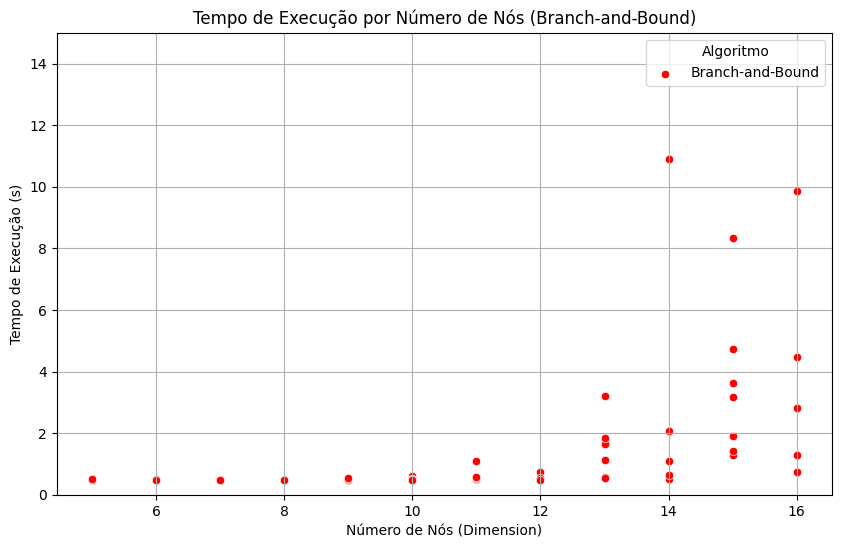
\includegraphics[width=.7\textwidth]{Figure6.png}
\caption{Gráfico Tempo de Execução por Número de Nós (Branch-And-Bound)}
\label{fig:exampleFig1}
\end{figure}

\subsection{Twice-Around-the-Tree (TATT)}
Com os resultados em mãos e gerando um gráfico de Tempo de Execução por Número de Nós (Figure 1), foi possível observar que o algoritmo Twice-Around-the-Tree apresentou desempenho consistente em relação ao tempo de execução, visto que, para instâncias menores, o tempo médio foi de 1.5 segundos. Entretanto, para instâncias maiores, o tempo aumentou de forma considerável, chegando a 109 segundos para o maior grafo testado, gerando uma media final de aproximadamente 7.27 segundos. Já em relação à qualidade, o TATT apresentou um fator de aproximação médio de 1.37, sendo o pior resultado 1.57, o que é esperado devido à garantia teórica do algoritmo.

\begin{figure}[ht]
\centering
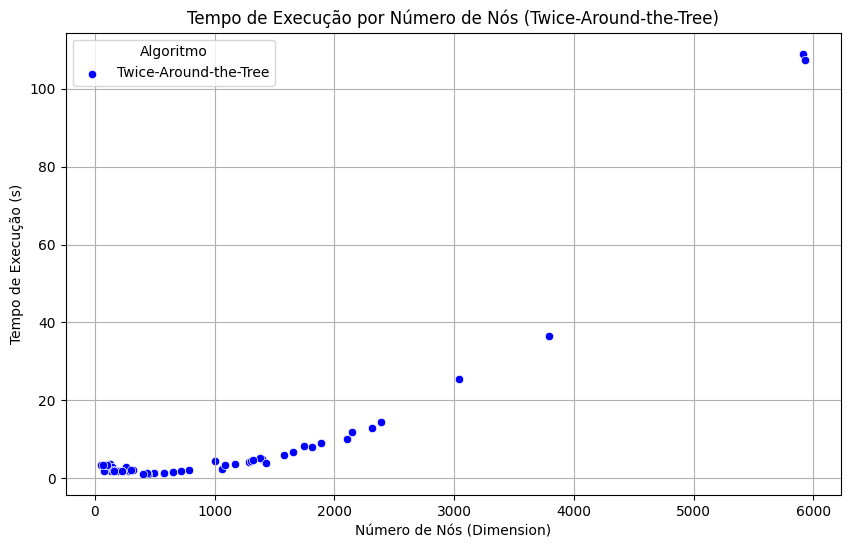
\includegraphics[width=.7\textwidth]{Figure1.png}
\caption{Gráfico Tempo de Execução por Número de Nós (TATT)}
\label{fig:exampleFig2}
\end{figure}

\subsection{Christofides}
O algoritmo Christofides (Figure 2), por sua vez, obteve um desempenho geral melhor no quesito qualidade da solução, apresentando um fator de aproximação médio de 1.12, com o pior resultado em 1.20. Entretanto, o tempo de execução para instâncias maiores foi consideravelmente superior ao do TATT, apresentando um tempo médio de 4 segundos para grafos menores, e até 553 segundos para instâncias maiores, gerando uma média geral de aproximadamente 46 segundos.

A análise reforça que, embora o Christofides tenha maior custo computacional, sua qualidade de solução é superior, o que o torna mais adequado para problemas onde a precisão da solução é um fator crítico.
\\
\\
\\
\\

\begin{figure}[ht]
\centering
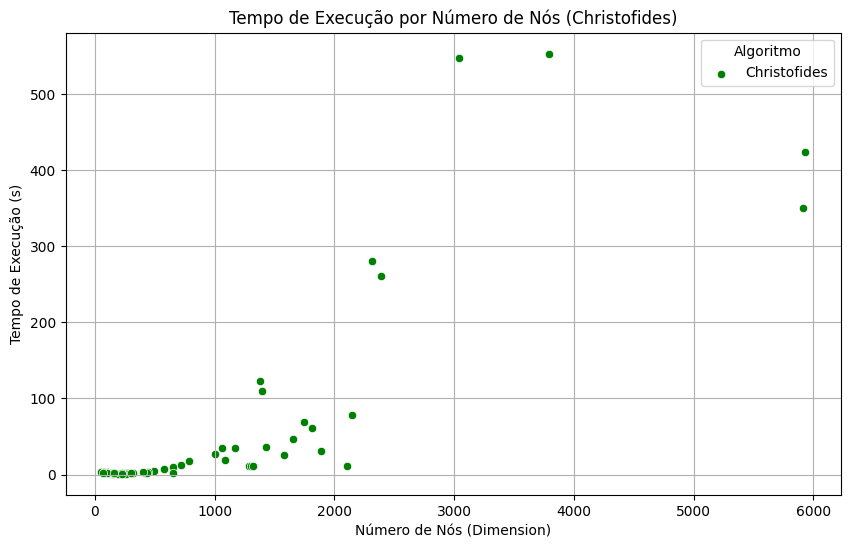
\includegraphics[width=.7\textwidth]{Figure2.png}
\caption{Gráfico Tempo de Execução por Número de Nós (Christofides)}
\label{fig:exampleFig3}
\end{figure}

\subsection{Comparação dos Algoritmos}
Os resultados comparativos entre os algoritmos estão sumarizados na Tabela~\ref{tab:comparison} e Tabela~\ref{tab:comparative_analysis}. Ao comparar os resultados, é possível observar que o TATT é mais eficiente em termos de tempo, porém sua qualidade da solução é inferior ao Christofides, já em termos de escalabilidade, ambos os algoritmos apresentaram comportamentos semelhantes, mas o Christofides mostrou-se mais limitado em relação ao tempo para instâncias maiores.

A partir dos dados coletados, também foi gerado um gráfico (Figure 4) que relaciona o número de vértices das instâncias com as métricas de tempo e qualidade. Nesse caso, foi possível notar que o Twice-Around-The-Tree mostrou-se mais eficiente em instâncias com maior número de vértices, apresentando tempos significativamente menores.
Já o Christofides, embora mais lento, apresentou crescimento de tempo alinhado com sua complexidade assintótica. Quanto à Qualidade da Solução, o Algoritmo de Christofides apresentou melhores resultados, com soluções mais próximas do ótimo em relação ao TATT. Quanto ao gasto de memória (Figure 5), é possível notar que ambos apresentaram resultados bem semelhantes.

\begin{figure}[ht]
\centering
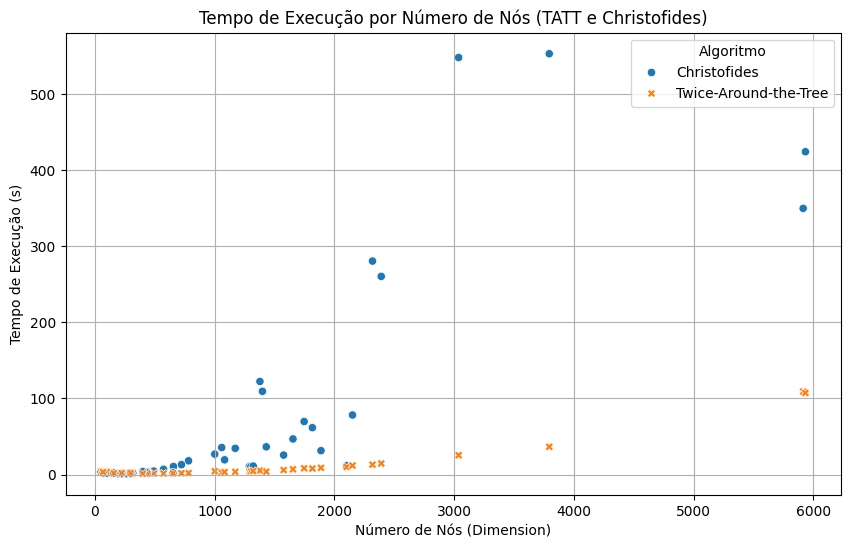
\includegraphics[width=.7\textwidth]{Figure3.png}
\caption{Comparativo - Tempo de Execução por Número de Nós (TATT e Christofides)}
\label{fig:exampleFig4}
\end{figure}

\begin{figure}[ht]
\centering
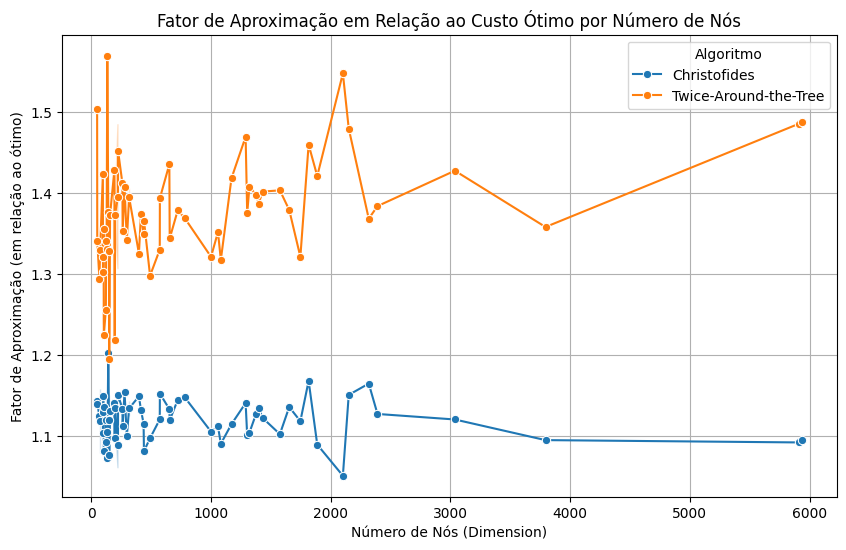
\includegraphics[width=.7\textwidth]{Figure4.png}
\caption{Comparativo - Fator de Aproximação (TATT e Christofides)}
\label{fig:exampleFig5}
\end{figure}

Portanto, é possível dizer que o algoritmo Twice-Around-the-Tree é mais eficiente em tempo, enquanto o Christofides se destaca em qualidade da solução. A escolha entre os dois depende da aplicação: o TATT é mais indicado para problemas onde o tempo de execução é crítico, enquanto o Christofides deve ser usado em problemas onde a qualidade da solução é o principal fator.

\begin{figure}[ht]
\centering
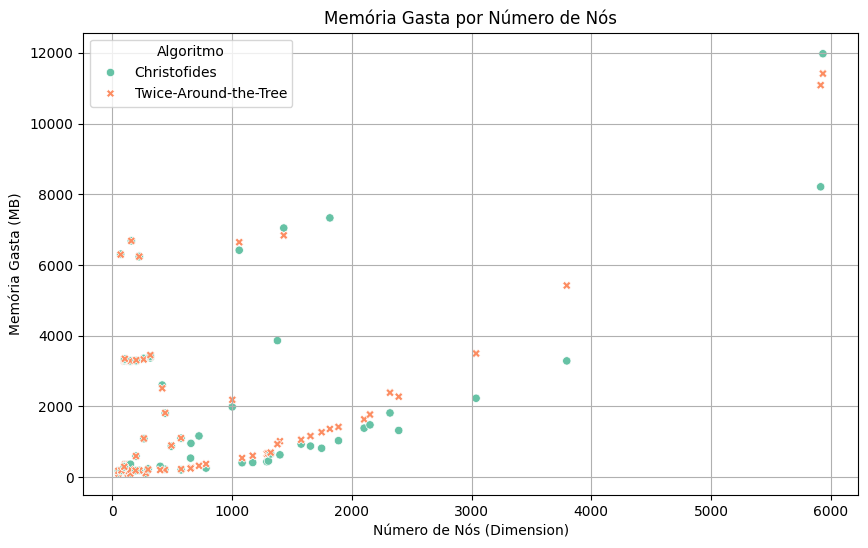
\includegraphics[width=.7\textwidth]{Figure5.png}
\caption{Comparativo - Fator de Aproximação (TATT e Christofides)}
\label{fig:exampleFig6}
\end{figure}

\section{Conclusão}

Neste trabalho, foram implementados e analisados três algoritmos para resolver o Problema do Caixeiro Viajante (TSP) em sua variação euclidiana: Branch-and-Bound, Twice-Around-the-Tree (TATT) e Christofides. Cada abordagem possui características específicas que as tornam adequadas para diferentes contextos e tamanhos de instâncias do problema.

O algoritmo Branch-and-Bound demonstrou ser uma solução exata eficiente para instâncias de menor porte, sendo capaz de garantir a solução ótima ao custo de uma complexidade exponencial. No entanto, sua aplicação prática é limitada devido ao rápido crescimento do espaço de busca, tornando-o impraticável para instâncias maiores, como evidenciado nos experimentos realizados.

Por outro lado, os algoritmos aproximados Twice-Around-the-Tree e Christofides apresentaram desempenhos significativamente superiores em termos de tempo de execução, mesmo para instâncias de maior porte. O TATT destacou-se pela simplicidade e baixa complexidade computacional, fornecendo soluções razoáveis de maneira eficiente. Já o algoritmo de Christofides, apesar de ser mais complexo, apresentou soluções de melhor qualidade com um fator de aproximação garantido de 1,5, tornando-se uma opção robusta para aplicações que requerem um equilíbrio entre qualidade e eficiência.

Os experimentos com as instâncias da TSPLIB confirmaram as propriedades teóricas dos algoritmos e permitiram comparar suas performances em um ambiente controlado. A escolha do algoritmo mais adequado depende, portanto, do contexto do problema, das restrições de tempo de execução e da qualidade esperada da solução. Para aplicações críticas, onde a solução ótima é essencial, o Branch-and-Bound pode ser viável em instâncias pequenas. Para problemas de maior escala ou quando uma solução aproximada de alta qualidade é aceitável, o algoritmo de Christofides é a alternativa mais apropriada.

\begin{thebibliography}{99}

\bibitem{dickson} 
DICKSON, G. \textit{Blossom Algorithm}. Disponível em: \url{https://www.eecs.tufts.edu/~gdicks02/Blossom/Blossom_Algorithm.html}. Acesso em: 07 jan. 2025.

\bibitem{networkx} 
NETWORKX DEVELOPERS. \textit{NetworkX Documentation}. Disponível em: \url{https://networkx.github.io/documentation/latest/index.html}. Acesso em: 07 jan. 2025.

\bibitem{igraph} 
IGRAH DEVELOPERS. \textit{iGraph}. Disponível em: \url{https://igraph.org}. Acesso em: 07 jan. 2025.

\bibitem{arbex} 
ARBEX, M. \textit{Escrita Científica}. Disponível em: \url{https://homepages.dcc.ufmg.br/~mirella/doku.php?id=escrita}. Acesso em: 13 jan. 2025.

\bibitem{tsplib} 
TSPLIB DEVELOPERS. \textit{TSPLIB}. Disponível em: \url{http://comopt.ifi.uni-heidelberg.de/software/TSPLIB95/}. Acesso em: 15 jan. 2025.
\\

\end{thebibliography}

\begin{table}[ht]
\centering
\caption{Comparação de Qualidade e Tempo entre Christofides e TATT}
\label{tab:comparison}
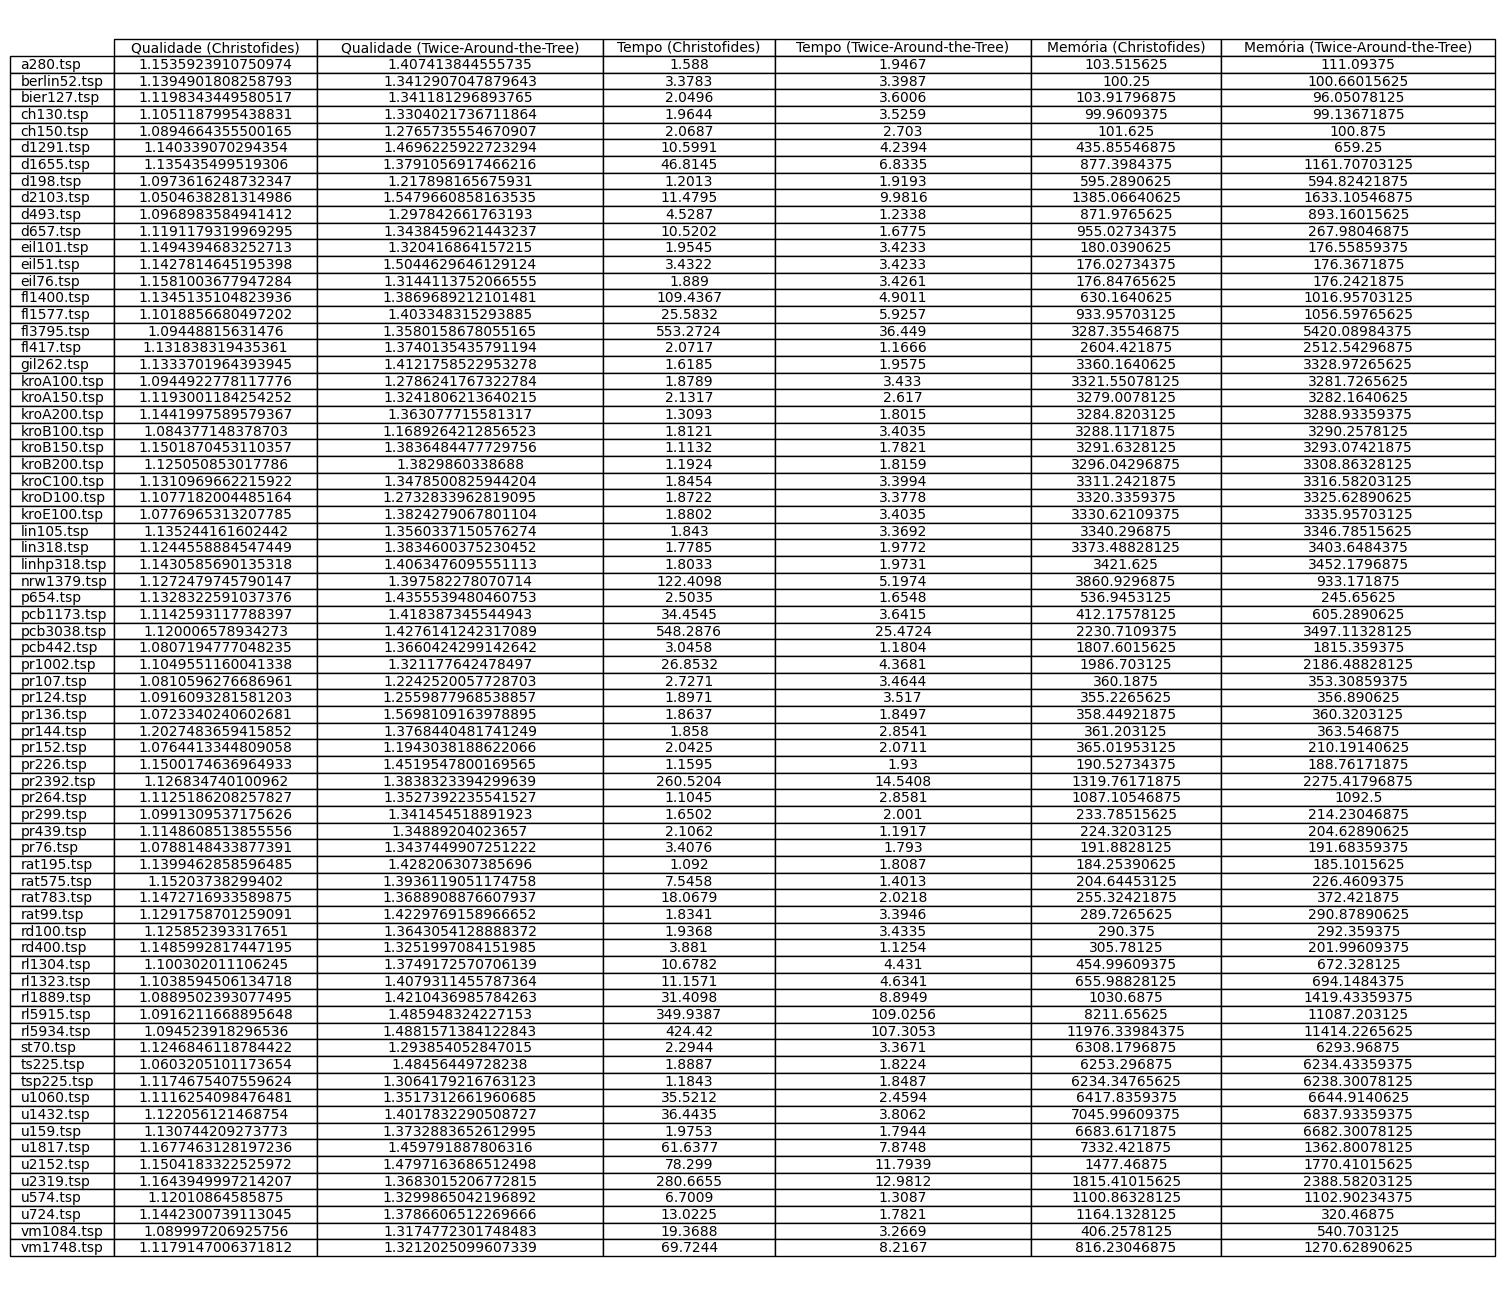
\includegraphics[width=1.1\textwidth]{Tabela1.png}
\end{table}

\begin{table}[ht]
\caption{Análise Comparativa entre os Algoritmos TATT e Christofides}
\label{tab:comparative_analysis}
\small % Reduz o tamanho da fonte
\begin{tabularx}{\textwidth}{lXXXX}
\toprule
Métrica & Min & Max & Média & Desvio Padrão \\
\midrule
Tempo de execução (s) - TATT & 1.125400 & 109.025600 & 7.270417 & 17.986843 \\
Tempo de execução (s) - Christofides & 1.092000 & 553.272400 & 45.895688 & 116.047413 \\
Qualidade da solução - TATT & 1.168926 & 1.569811 & 1.369944 & 0.074386 \\
Qualidade da solução - Christofides & 1.050464 & 1.202748 & 1.118898 & 0.027803 \\
Memória Gasta - TATT & 96.050781 & 11414.226 & 2071.492 & 2463.333 \\
Memória Gasta - Christofides & 99.960938 & 11976.340 & 2078.278 & 2422.928 \\
\bottomrule
\end{tabularx}
\end{table}

\end{document}
